\part{Telemetry System Design}

This year's telemetry system aims to address the shortcomings in last year's design. The main flaws that are being
addressed are:

\begin{itemize}
    \item Battery life status updates
    \item Power consumption
    \item System size for physical placement in the rocket
    \item Radio signal strength
    \item Enclosure integrity under shock load
    \item Lack of sensor fusion and equal data acquisition
    \item Use of memory for data logging while the rocket is idle
\end{itemize}

\section{Hardware Design}

\subsection{Power System}

\fxwarning{Add power system and arming design}

\subsection{Sensor Systems}

\fxwarning{Add sensor systems design}

\section{Radio Frequency Design}

The radio transmitter portion of the telemetry system will be based on a student-designed \gls{pcb} designed around the
RN2483 radio transceiver chip. More information about the chip's specifications can be found in Appendix
\ref{apx:rn483}. You can see the chip featured on the Pictail board in Figure \ref{fig:pictail}

\begin{figure}[H]
    \centering
    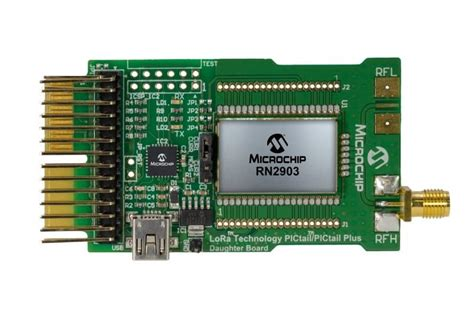
\includegraphics[width=3in]{assets/images/pictail.jpg}
    \caption{The RN2483 radio transceiver chip on the commercial Pictail board \cite{pictail-img}}
    \label{fig:pictail}
\end{figure}

The RN2483 chip was selected because of its low power consumption of 38.9 milliamps when transmitting \cite[Table
    2-3]{rn2483-datasheet} and long-range capabilities, transmitting up to a distance of 15 kilometres in suburban
environments \cite[1]{rn2483-datasheet}. It also has a \gls{cots} twin, the RN2483 Pictail board. This is useful to
compare our \gls{srad} designs against during range testing.

\subsection{Radio Parameters}

\subsubsection{Frequency}

The RN2483 transceiver will be used to operate on the 433MHz band in our systems. This frequency band was selected
because it requires a lower transmit power for the same range \cite[Table 2-5]{rn2483-datasheet} as the 868MHz band.
This band is also licensed as a \gls{ham-radio} band. \Gls{cuinspace} has amateur radio certified members who can
operate our radio systems and provide their call-sign for use in the transmissions. Our exact frequency is 433.5MHz.

\subsubsection{Modulation}

The RN2483 is capable of both FSK and LoRa modulation, but InSpace will be using LoRa modulation since it provides
better long-range performance. The modulation technique makes signals less susceptible to noise.

\subsubsection{Spread Factor}

The spread factor determines how much the signal is spread across the frequency band used by the radio. It is possible
to set spread factors from 7 to 12. \cite[Sec. 2.5.5.14]{rn2483-commands} A lower spread factor increases data rate.

\Gls{cuinspace} uses the lowest spread factor of 7 to maximize the data rate.

\subsection{PCB Design Considerations}

The radio board is designed to be a four layer \gls{pcb}. This allows top and bottom copper signal routing, with ground
and power planes in the center.

The ground plane will be layer immediately under the top copper, as it provides a reference plane which is beneficial
for radio frequency traces. The trace will be a microstrip line, which is a copper trace running above a ground plane,
separated by an impedance controlled dielectric. A visual of microstrip can be seen in Figure \ref{fig:microstrip}.

\begin{figure}[H]
    \centering
    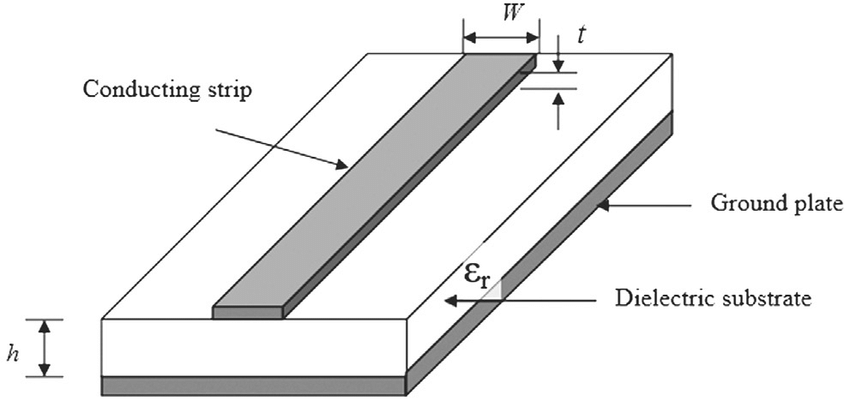
\includegraphics[width=3in]{assets/images/microstrip.png}
    \caption{Microstrip line \cite{microstrip}}
    \label{fig:microstrip}
\end{figure}

Our radio frequency traces are impedance controlled to 50 ohms, which is a standard impedance for radio equipment,
including the \gls{sma} connectors and antennas used by \gls{cuinspace}.

All radio frequency traces on the board are also kept below the critical length for the 433MHz frequency, which
prevents them from acting as an antenna themselves. \Gls{pcb} trace lengths should not exceed 1/12th of the wavelength
in the dielectric. \cite{critical-length}

Our manufacturer's dielectric constant for the prepreg layer we use on our impedance controlled boards is 4.4.
\cite{jlc-pcb-impedance}. Equation \ref{eq:wavelength} is used to calculate the wavelength of the radio signal in the
PCB trace.

\begin{equation}
    \lambda = \frac{c}{f\sqrt{\epsilon_R}}
\end{equation} \label{eq:wavelength}

Then, given this wavelength, the critical length is calculated using Equation \ref{eq:critlen}.

\begin{equation}
    L = \frac{1}{12} \times \lambda
\end{equation} \label{eq:critlen}

The critical length of the trace for our operating frequency of 433.5MHz is approximately 2.75 centimetres. All of our
\gls{rf} traces carrying 433.5MHz signals will therefore be designed to have a total length less than 2.75 centimetres.

\begin{gather*}
    \lambda = \frac{300 \times 10^6}{(433.5 \times 10^6)\sqrt{4.4}} \\
    \lambda = 0.32991785095003 \\
    \\
    L = \frac{1}{12} \times (0.32991785095003) \\
    L = 0.027493154245836 \\
    L \approx 0.0275 \\
\end{gather*}

In addition, our \gls{rf} traces will be designed to have no sharp bends. The RN2483 sample application show traces
that have two bends with a radius of 2.0 millimetres. \cite[Sec. 5.1]{rn2483-datasheet} If a bend is necessary, the
design will adhere to this bend radius.

\section{Real-Time Operating System}

The telemetry transmitter will run a \gls{rtos} called Apache NuttX (referred to as NuttX from here onward). NuttX is
an embedded \gls{rtos} which is designed to have an incredibly small footprint through its many configuration options.
\cite{nuttx-about}. It is \gls{posix} compliant and also adheres to several other standards in the embedded systems
space for APIs that are not governed by \gls{posix}. \cite{nuttx-about} It's completely open source under the Apache
2.0 license and provides a host of existing tools and drivers for file systems, memory devices, analog devices and
digital sensors/peripherals. NuttX has an open community forum for getting support and reporting bugs, which has been
an asset during development. \Gls{cuinspace} is also able to contribute driver code back to the project for the benefit
of others, and has been doing so.

\subsection{Driver Code}

Drivers in NuttX are interacted with via a POSIX interface, composed primarily of the following standard functions:

\begin{itemize}
    \item \texttt{open(const char *path, int oflag, ...)}
    \item \texttt{close(int fildes)}
    \item \texttt{read(int fildes, void *buf, size\_t nbyte)}
    \item \texttt{write(int fildes, void *buf, size\_t nbyte)}
    \item \texttt{ioctl(int fildes, int request, ...)}
\end{itemize}

This allows devices to be interacted with through the regular path name space, just like files. This is standard for
Unix systems, and makes writing application code incredibly convenient.

A major benefit of NuttX's \gls{posix} interface is code portability. By abstracting away low-level code through
drivers which act as files, application code can run on any other \gls{posix} system. This opens up testing
possibilities that allow developers to write and debug application code on their own Linux/MacOS machines before
flashing the microcontroller.

NuttX also supplies drivers of its own for very standard communication protocols such as \gls{uart}, \gls{i2c},
\gls{spi}, etc. This facilitates the writing of device drivers for simple digital sensors such as an \gls{imu} or
temperature sensor.

\subsection{Scheduling}

Task scheduling within NuttX can be easily performed using \gls{posix} \glspl{api} again. It is possible to create
multiple processes or threads which are scheduled by the operating system using a methodology chosen by the developer
(first-in-first-out, round robin, etc.). This also allows \gls{io} operations to be performed alongside the processor
performing application logic.

\Gls{cuinspace} will be leveraging scheduling features to write multi-threaded programs. This allows us to split tasks
by priority and ensure that the highest priority tasks are given time in the processor. In the case of the telemetry
system, highest priority will be given to data logging and radio transmission operations, since those require very
little processor time and only have to trigger short bursts of \gls{io} operations.

\textbf{Task priorities from highest to lowest:}

\begin{enumerate}
    \item SD card logging
    \item Radio transmission
    \item Sensor data collection
    \item Packet encoding
\end{enumerate}

Packet encoding is the most \gls{cpu} intensive task but is also lowest priority since the \gls{io} operations are
critical and take very little \gls{cpu} time, so they can afford to be ushered in to quickly trigger an \gls{io}
operation and relinquish the \gls{cpu}.

The telemetry system will immediately perform boot operations to load all the device drivers before launching into the
application code at power-on.

\section{Data Delivery}

Data logging during flight will be done in a significantly more robust manner than previous years. This involves more
physically secure memory for logging, as well as power-failure guarantees. \Gls{cuinspace} will also be conserving
space through lift-off and landing detection.

Data transmission has worked reliably from a protocol standpoint, and the previous design will be continued and
expanded upon.

\subsection{Data Log Integrity}

The physical memory being used for flight data logging is a standard microSD card. This memory was chosen because it is
cheap, ubiquitous, has an extremely large capacity and is easy to remove for data analysis on a computer immediately
after the rocket is recovered.

One of the challenges posed by an SD card is that it is designed to be removable in nature. SD card slots for quick
removal do not fare well in high vibration and high shock force environments like a rocket. They create a risk for the
SD card to fall out in flight, and also an opportunity for vibrations to temporarily break the electrical connection
between the card and the \gls{mcu}.

To address these risks, \gls{cuinspace} is securing the SD card in a cage-like slot, specifically manufactured to
survive shock loads of up to 50g and have electronic discontinuity for only up to 1 microsecond.
\cite{sd-cage-datasheet} An image of this microSD slot can be seen in \Cref{fig:sd-card-cage}.

\begin{figure}[H]
    \centering
    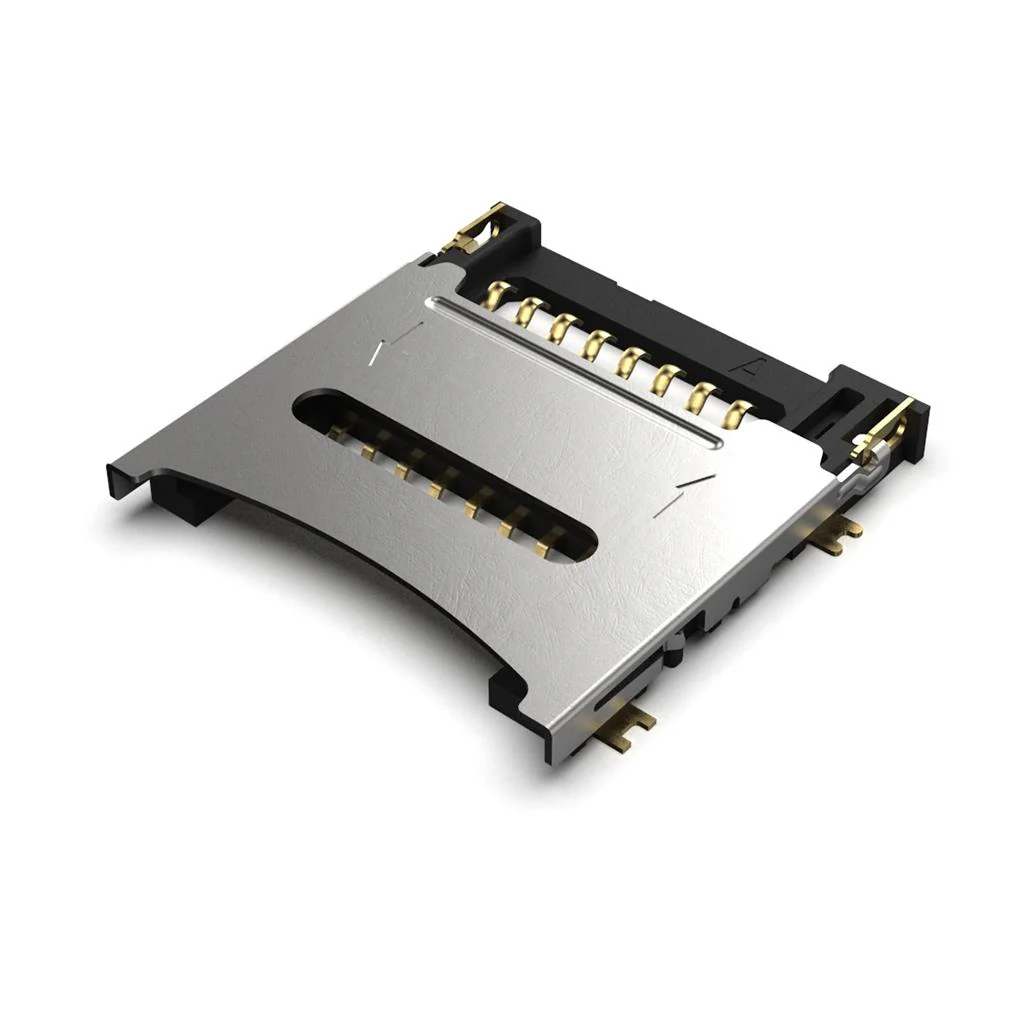
\includegraphics[width=2in]{./assets/images/sd-card-cage.png}
    \caption{Shock load resistant microSD card slot \cite{sd-card-cage}}
    \label{fig:sd-card-cage}
\end{figure}

In order to mitigate discontinuity risks on the software side, the microSD card will make use of the \textit{littlefs}
file system, which provides power-failure safety guarantees. Any brief discontinuity during a write to the SD card will
not corrupt any data, thus preserving the integrity of all logs. You can read more about \textit{littlefs} in
\Cref{apx:littlefs}.

In addition to the \textit{littlefs} file system on the microSD card, there will also be a FAT file system partition.
This partition allows for easy viewing of the telemetry data on a laptop immediately after recovery, as the FAT file
system is accessible through the file explorer on both Windows and Linux computers. Logged flight data is copied from
the \textit{littlefs} partition to the FAT partition upon landing, when there is very little risk of vibrations
corrupting the transfer. The FAT partition will be the first partition on the microSD's partition table so that it is
detected properly on Windows machines.

\subsection{Logging Space Conservation}

In order to preserve logging space and avoid filling up memory with telemetry data being collected while the rocket is
idle on the launch rail, we will be using lift-off and landing detection to trigger logging operations. The \gls{fsm}
used to govern this portion of the system can be seen in \Cref{fig:logging-fsm}.

\begin{figure}[H]
    \centering
    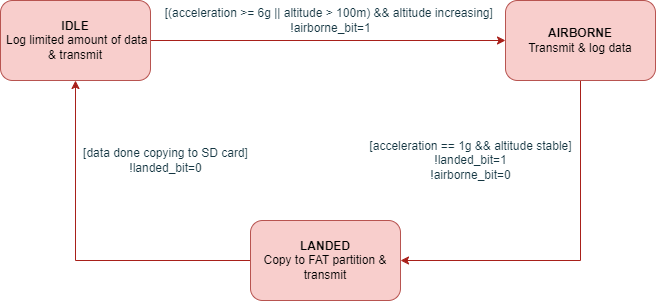
\includegraphics[width=4in]{./assets/diagrams/Flight State FSM.png}
    \caption{Logging control \gls{fsm}}
    \label{fig:logging-fsm}
\end{figure}

Last year, much of the logged telemetry data was captured while the rocket was idle on the launch rail. This is the
\textit{IDLE} state in \Cref{fig:logging-fsm}. In this state we continue to transmit telemetry because it's necessary
to confirm the system's operation and a stable radio signal, but we do not log continuously. Instead, logs are recorded
for only the past 30 seconds at any given time. This gives the system breathing room for latency when detecting
lift-off, without losing any critical data about the start of the launch.

Lift-off is detected using the accelerometer data in conjunction with the barometric pressure sensor. The accelerometer
data can detect the high g-force experienced at launch (previous launches have seen up to 24g) and the barometric
pressure sensor can detect a climbing altitude. In the first few seconds of lift-off, the system will be able to detect
the high g-force and increasing acceleration, at which point it will move to the \textit{AIRBORNE} state. This state is
recorded by setting the "airborne bit" to 1 in the on-board \gls{eeprom}. Doing so means that if the system experience
power-failure in the air, when it reboots it will successfully boot into the \textit{AIRBORNE} state again.

In the \textit{AIRBORNE} state, the flight computer will continuously log to the \textit{littlefs} partition on the SD
card. This will capture flight data at a much higher frequency than is possible to transmit over radio.

Eventually, once the rocket has deployed its chutes at apogee and descended to the ground, the system will detect
landing. The criteria for landing detection is an accelerometer reading of maximum 1g (with slight tolerance for noise)
in any axes combined with a stable altitude which is at ground level. This should prevent landing detection from
triggering while the rocket is at apogee or descending slowly, at which point its altitude will still be quite high and
it should be descending at a larger acceleration than 1g. These thresholds will be configurable and will be set prior
to flight based on simulations on descent speed by the recovery team.

Once the landing is detected, the system will enter the \textit{LANDED} state. In this state the "airborne bit" will be
set to 0 and the "landed bit" will be set to 1. The system will begin copying all logged flight data from the
\textit{littlefs} partition to the FAT file system partition on the SD card. During this time it continues to transmit
telemetry over radio.

Once all the data is copied over, the "landed bit" will be set to 0, and the system will re-enter the \textit{IDLE}
state. At this point, the system still continues transmitting GPS coordinates for recovery, and all flight logs are
safe on the SD card for post-flight extraction. Logs on the \textit{littlefs} partition are only over-written when the
system re-enters the \textit{AIRBORNE} state, which is not possible to trigger from the ground.

\subsection{Data Transmission}

The other method in which \gls{cuinspace} records telemetry data is via live radio broadcasting while the radio is in
flight. This allows a downlink ground station to receive real-time updates about the rocket state while it is in-
flight.

In order to transmit telemetry data over radio, \gls{cuinspace} has developed a radio packet encoding format. This
format can be found in Appendix \ref{apx:comm-spec-repos}. The format covers multiple different data types that are
recorded about the rocket state, such as altitude, acceleration, \gls{gps} coordinates, etc. \cite{radio-comms}.
Importantly, each radio packet starts with a header containing the amateur radio call-sign of the \gls{cuinspace}
operator responsible for flying the system. \cite{radio-comms} The original specification did not include sufficient
space to append a call-zone indicator to the call-sign, which has since been amended in the latest version. This is a
requirement for Canadians broadcasting in the United States \cite{foreign-broadcast}, as \gls{cuinspace} does at
\gls{sac}.

Since \gls{cuinspace}'s rockets achieve altitudes up to around 9 kilometres, it is necessary to choose a radio unit
that can transmit up to such a long range. Unfortunately, long range transmissions are achieved with a trade-off in
bandwidth. This means that the radio unit is not always able to match the measurement speed of the telemetry system.
The on-board data logging is fast enough to capture the full resolution of measured data, but since the radio has low
bandwidth, it is only used to broadcast the most recently measured packet at the time when it becomes ready for another
transmission.

\section{Enclosure Design}

%This might be in aerostructures PDR, not certain.
